\documentclass{ctexbeamer}        % 文档类beamer的汉化版本
%\documentclass{beamer}

\usefonttheme{serif}              % 使用衬线字体
\usefonttheme{professionalfonts}  % 数学公式字体

\usepackage{mathtools}
\usepackage{graphicx}
\usepackage{xcolor}
\usepackage{amsfonts}
\usepackage{amssymb}
\usepackage{bbm}
\usepackage{tcolorbox}
\usepackage{listings}
\usepackage{amsmath}
\usepackage{enumerate}
\usepackage{bbold}
\usepackage{bm}
\usepackage[ruled,linesnumbered]{algorithm2e}
\usepackage{mathtools}

\setbeamertemplate{frametitle continuation}[from second][]
%% --> 配置中英文字体
% \usepackage{fontspec}
% \setmainfont{Liberation Serif}
% \setsansfont{DejaVu Sans}
% \setmonofont{Cousine}
% \usepackage{xeCJK}
% \setCJKmainfont[BoldFont=Noto Sans SC]{Noto Serif SC}
% \setCJKsansfont{Noto Sans SC}
% \setCJKmonofont{WenQuanYi Micro Hei Mono}

%% --> 主题和色彩风格
\usetheme{Frankfurt}
\usecolortheme{whale}
\definecolor{lightyellow}{HTML}{F5F5DC}
\definecolor{lightgrey}{HTML}{FF8C69}
\lstset{language=Python,
        basicstyle=\ttfamily\bfseries,
        commentstyle=\color{red}\itshape,
        stringstyle=\color{darkgreen},
        showstringspaces=false,
        keywordstyle=\color{blue}\bfseries,
        basicstyle=\scriptsize,
        frame=shadowbox}


\newtheorem{theorem_}{定理}
\newtheorem{proof_}{证明}
\begin{document}
\title{决策树}
\author{耿远昊}
\institute{Datawhale}
\date{\today}
\frame{\titlepage}


%\begin{frame}{章节内容}
%  \tableofcontents[hideallsubsections]
%\end{frame}

\AtBeginSection[]{\frame{\tableofcontents[currentsection,hideallsubsections]}}

\section{信息论基础}

\begin{frame}{信息论基础}
树具有天然的分支结构。对于分类问题而言,决策树的思想是用节点代表样本集合,通过某些判定条件来对节点内的样本进行分配,将它们划分到该节点下的子节点,并且要求各个子节点中类别的纯度之和应高于该节点中的类别纯度,从而起到分类效果。
\newline

节点纯度反映的是节点样本标签的不确定性。当一个节点的纯度较低时,说明每种类别都倾向于以比较均匀的频率出现,从而我们较难在这个节点上得到关于样本标签的具体信息,其不确定性较高。当一个节点的纯度很高时,说明有些类别倾向于以比较高的频率出现,从而我们能够更有信心地把握这个节点样本标签的具体信息,即确定性较高。
\end{frame}

\begin{frame}{信息论基础}
为了定义纯度的概念,我们首先需要思考如何度量不确定性。在生活中,高概率事件代表的不确定性比低概率事件代表的不确定性低,例如:明天太阳从东边升起是必然的,故这个事件的不确定性为0;而明天下雨并不是必然事件,它相比前一个事件具有更高的不确定性。因此,若定义一个可微函数$I(p),p\in [0, 1]$来表示事件$A$发生的概率$p(A)$所代表的不确定性,那么从直觉上应当满足下面三个必要条件,我们将它们称为信息量公理。其中,$A_1,...,A_n$为独立事件。

\begin{enumerate}
\item $I(1)=0$
\item $I(p)$关于$p$单调递减
\item $I(\prod_{i=1}^np(A_i))=\sum_{i=1}^nI(p(A_i))$
\end{enumerate}
\end{frame}

\begin{frame}{信息论基础}
我们已经对信息量公理的前两个条件做出了说明,其第三个条件的含义是:独立事件同时发生的不确定性应当等于这些事件对应发生的不确定性之和,这是非常合理的假设。
\newline

根据这些条件,我们容易想到函数
$$
I(p)=a\log_{b}(p)(a(b-1)<0)
$$
符合信息量公理的要求。事实上从充分性的角度而言,它也是能够满足信息量公理的唯一函数。
\end{frame}

\begin{frame}{信息论基础}
%\begin{tcolorbox}[colback=lightyellow,colframe=lightgrey,title=\color{black}{定理}]
%  	设$I(p)$在$[0,1]$上可微,则$I(x)$满足信息量公理的充要条件是 $I(p)=a\log_{b}(p)(a(b-1)<0)$。
%\end{tcolorbox}
\begin{theorem_}
设$I(p)$在$[0,1]$上可微,则$I(x)$满足信息量公理的充要条件是 $I(p)=a\log_{b}(p)(a(b-1)<0)$。
\end{theorem_}
\begin{proof_}
当$x\in (0,1]$,此时由导数定义有
\begin{align*}
I^{'}(x) &= \lim_{\Delta x\rightarrow 0^-}\frac{I(x+\Delta x)-I(x)}{\Delta x} \\
&= \lim_{\Delta x\rightarrow 0^-}\frac{I(\frac{x+\Delta x}{x}\cdot x)-I(x)}{\Delta x} 
\end{align*}
\end{proof_}

\end{frame}
\begin{frame}{信息论基础}
\begin{proof_}[续]
$$
I^{'}(x)= \lim_{\Delta x\rightarrow 0^-}\frac{I(\frac{x+\Delta x}{x})}{\Delta x}= \frac{1}{x}\lim_{\Delta x\rightarrow 0^-}\frac{I(1+\frac{\Delta x}{x})}{\frac{\Delta x}{x}} = \frac{1}{x}I^{'}(1)
$$
两边积分$I(x)=I^{'}(1)\ln x+C,x\in(0,1]$,代入$I(1)=0$得$C=0$,从而
$$
I(x)=I^{'}(1)\ln(x)=\frac{I^{'}(1)}{\log_be}\log_bx
$$
记$a=\frac{I^{'}(1)}{\log_be}$,由单调性可知$I^{'}(1)<0$。当$b>1$时有$\log_be>0$,即$a<0$;当$b<1$时有$\log_be<0$,即$a>0$。因此,符合信息量公理的函数只能是$I(p)=a\log_{b}(p)(a(b-1)<0)$。
\end{proof_}
\end{frame}
\begin{frame}{信息论基础}
我们已经知道了信息量对应函数的形式,那么究竟应该如何选取合适的$a$和$b$呢?对于一个以概率为$p$发生的事件$A$而言,我们可以选择一种二进制编码的方式来记录它的信息:当$p=\frac{1}{4}$时,我们可以认为事件$A$的发生本质上是某个随机变量的一种状态,且该随机变量会以等概率出现4种状态,那么我们就可以用00、01、10和11来进行状态信息的记录;当$p=\frac{1}{8}$时,我们需要用000、001、010、011、100、101、110、111的编码来记录。因此,$p$越小则不确定性越高,需要消耗的编码长度越大。此时,编码种类的数量即为$\frac{1}{p}$,事件$A$的二进制编码长度代表的不确定性大小就是$\log_2\frac{1}{p}$。因此,我们可以取$I(p)$中的$a$为$-1$,且取$b$为$2$,用$I(p)=-\log_2(p)$来代表度量不确定性的指标。
\end{frame}

\begin{frame}{信息论基础}
先前我们讨论了随机变量取定某个值情况下不确定性的度量,那么如果要定义一个随机变量$X$的平均不确定性,只需要对这个随机变量按照对应的概率密度分布$p(x)$取期望即可,我们将其称为分布的信息熵(Information Entropy)$H(X)$(熵是一种反应系统不确定性的指标,由于此处指随机变量信息的不确定性,故称为信息熵),即
$$
H(X)=\mathbbm{E}_{X}I(p)=\mathbbm{E}_{X\sim p(x)}[-\log_2 p(X)]
$$
对于定义在有限状态集合$\{x_1,...,x_K\}$上的离散变量而言,对应信息熵的最大值在离散均匀分布时取到,最小值在单点分布时取到。此时,离散信息熵为
$$
H(X)=-\sum_{k=1}^K p(x_k)\log_2p(x_k)
$$
\end{frame}

\begin{frame}{信息论基础}
首先,我们需要定义当$p$时$p\log_2p\triangleq 0$,原因在于
$$
\lim \limits_{p\to 0^+} p \log{p} = \lim \limits_{p \to 0^+} \frac{\log p}{1/p} = \lim \limits_{p \to 0^+} \frac{1/p}{-1/p^2}=\lim \limits_{p \to 0^+} -p = 0
$$
离散熵的极值问题是带有约束的极值问题,记$p_k=P(X=x_k)$和$\mathbf{p}=[p_1,...,p_K]^T$,则约束条件为$\mathbbm{1}^T\mathbf{p}=1$,拉格朗日函数为
$$
L(\mathbf{p})=-\mathbf{p}^T\log \mathbf{p} + \lambda (\mathbbm{1}^T\mathbf{p}-1)
$$
求偏导数后可解得$\mathbf{p}^*=[\frac{1}{K},...,\frac{1}{K}]$,此时$\mathbbm{E}_{X}I(p)=\log K$。
\end{frame}

\begin{frame}{信息论基础}
对于离散随机变量$X$,由于$p(X)\in [0,1]$,故$-\log_2p(X)\geq 0$,从而$\mathbbm{E}_{X}I(p)\geq 0$。注意到对于$\forall k\in \{1,...,K\}$,当$p_k=1$,即$p_{k'}=0(k'\in \{1,...,K\}/k)$时,$H(X)=0$。因此,离散信息熵的最小值为0且在单点分布时取到。由于$\mathbf{p}^*$是极值问题的唯一解,因此离散熵的最大值为$\log K$且在离散均匀分布时取到。
\newline

这些结论都是与直觉高度吻合的。单点分布的取值被唯一确定,因此随机变量的不确定性为0;在给定状态集合数量下,分布越是均匀,则随机变量的不确定性越是大;当$K\rightarrow +\infty$时,离散均匀分布的熵为无穷大,一个合理的解释是:随着取值集合元素数量的增加,我们对每一个元素平均而言的信息把握程度就越少,不确定性就越大。
\end{frame}

\begin{frame}{信息论基础}
由于在决策树的分裂过程中,我们不但需要考察本节点的不确定性或纯度,而且还要考察子节点的平均不确定性或平均纯度来决定是否进行分裂。子节点的产生来源于决策树分支的条件,因此我们不但要研究随机变量的信息熵,还要研究在给定条件下随机变量的平均信息熵或条件熵(Conditional Entropy)。从名字上看,条件熵就是条件分布的不确定性,那么自然可以如下定义条件熵$H(X\vert Y)$为
$$
\mathbbm{E}_{Y}[\mathbbm{E}_{X\vert Y}[-\log_2p(X\vert Y)]]
$$
对于离散条件熵,设$Y$所有可能的取值为$\{y_1,...,y_M\}$,上式可展开为
$$
-\sum_{m=1}^Mp(y_m)\sum_{k=1}^K p(x_k\vert Y=y_m)\log_2p(x_k\vert Y=y_m)
$$
\end{frame}

\begin{frame}{信息论基础}
有了信息熵和条件熵的基础,我们就能很自然地定义信息增益(Information Gain),即节点分裂之后带来了多少不确定性的降低或纯度的提高。当给定随机变量$Y$的取值$y$时,随机变量$X$的不确定性减少量为
$$
G(X,Y)=H(X)-H(X\vert Y)
$$
从直觉上说,随机变量$X$的信息增益一定是非负的,因为我们额外地知道了随机变量$Y$的取值,这个条件降低了$X$的不确定性。下面我们就从数学角度来证明其正确性。
\end{frame}

\begin{frame}{信息论基础}
\begin{align*}
G(X,Y)&=\mathbbm{E}_{X}[-\log_2p(X)]-\mathbbm{E}_{Y}[\mathbbm{E}_{X\vert Y}[-\log_2p(X\vert Y)]]\\
&=-\sum_{k=1}^Kp(x_k)\log_2p(x_k) \\
&\qquad+\sum_{m=1}^Mp(y_m)\sum_{k=1}^K p(x_k\vert Y=y_m)\log_2p(x_k\vert Y=y_m) \\
&=-\sum_{k=1}^K[\sum_{m=1}^Mp(x_k, y_m)]\log_2p(x_k) \\
&\qquad+\sum_{k=1}^K\sum_{m=1}^M p(y_m)\frac{p(x_k, y_m)}{p(y_m)}\log_2\frac{p(x_k, y_m)}{p(y_m)}
\end{align*}
\end{frame}
\begin{frame}{信息论基础}
\begin{align*}
G(X,Y)&=\sum_{k=1}^K\sum_{m=1}^Mp(x_k,y_m)[\log_2\frac{p(x_k, y_m)}{p(y_m)}-\log_2p(x_k)] \\
&=-\sum_{k=1}^K\sum_{m=1}^M p(x_k,y_m) \log\frac{p(x_k)p(y_m)}{p(x_k, y_m)}
\end{align*}
上式说明信息增益$G(X,Y)$就是$p(x,y)$和$p(x)p(y)$的KL散度,而KL散度的非负性由Jensen不等式可得:
\begin{align*}
G(X,Y)&\geq -\log_2 [\sum_{k=1}^K\sum_{m=1}^M p(x_k,y_m)\frac{p(x_k)p(y_m)}{p(x_k, y_m)}]\\
&= -\log_2 [\sum_{k=1}^K\sum_{m=1}^Mp(x_k,y_m)] = 0
\end{align*}
\end{frame}

\begin{frame}{信息论基础}
上式的取等条件为$p(x,y)=p(x)p(y)$,其实际意义为随机变量$X$和$Y$独立。这个条件同样与直觉相符合,因为如果$X$和$Y$独立,那么意味着我们无论是否知道$Y$的信息,都不会对$X$的不确定性产生影响,此时信息增益为0。
\newline

用信息增益的大小来进行决策树的节点分裂时,由于真实的分布函数未知,故用$p(x)$和$p(x\vert y)$的经验分布(即频率)来进行概率的估计。若节点$N$每个分支下的样本数量为$D_1,...,D_M$,记$\tilde{p}(y_m)=\frac{D_m}{\sum_{m'=1}^M D_{m'}}(m\in\{1,...,M\})$,$\tilde{p}(x_k)$和$\tilde{p}(x_k\vert y_m)$分别为节点中第k个类别的样本占节点总样本的比例和第m个子节点中第k个类别的样本数量占该子节点总样本的比例,则节点$N$分裂的信息增益定义为
{\small
$$
G_N(X,Y)=-\sum_{i=1}^K\tilde{p}(x_k)\log \tilde{p}(x_k)+\sum_{m=1}^M\tilde{p}(y_m)\sum_{k=1}^K\tilde{p}(x_k\vert y_m)\log_2 \tilde{p}(x_k\vert y_m)
$$
}

\end{frame}

\section{分类树的节点分裂}

\begin{frame}{分类树的节点分裂}
对于每个节点进行分裂决策时,我们会抽出max\_features个特征进行遍历以比较信息增益的大小。特征的类别可以分为三种情况讨论:类别特征、数值特征和含缺失值的特征,它们各自的处理方法略有不同。
\newline

对于类别特征而言,给定一个阈值$\epsilon$,树的每一个节点会选择最大信息增益$G^{max}_N(X,Y)$对应的特征进行分裂,直到所有节点的相对最大信息增益$\frac{D_N}{D_{all}}G^{max}_N(X,Y)$小于$\epsilon$,$D_N$和$D_{all}$分别指节点$N$的样本个数和整个数据集的样本个数,这种生成算法称为ID3算法。在sklearn中,$\epsilon$即为min\_impurity\_decrease。
\end{frame}

\begin{frame}{分类树的节点分裂}
C4.5算法在ID3算法的基础上做出了诸多改进,包括但不限于:处理数值特征、处理含缺失值的特征、使用信息增益比代替信息增益、提出处理带权样本的方法以及给出树的剪枝策略。其中,剪枝策略将在第4节进行讲解,下面先对前4个改进的细节来进行介绍。
\newline

在处理节点数值特征时,可以用两种方法来将数值特征通过分割转化为类别,它们分别是最佳分割法和随机分割法,分别对应了sklearn中splitter参数的best选项和random选项。
\newline

随机分割法下,取$s\sim U[y_{min}, y_{max}]$,其中$U[y_{min}, y_{max}]$代表特征最小值和最大值范围上的均匀分布,将节点样本按照特征$\mathbf{y}$中的元素是否超过$s$把样本划分为两个集合,这等价于把数值变量转换为了类别变量。此时,根据这两个类别来计算树节点分裂的信息增益,并将它作为这个数值特征分裂的信息增益。
\end{frame}

\begin{frame}{分类树的节点分裂}
最佳分割法下,依次令$s$取遍所有的$y_i(i=1,...,D_N)$,将其作为分割点,按照特征$\mathbf{y}$中的元素是否超过$s$把样本划分为两个集合,计算所有$s$对应信息增益的最大值,并将其作为这个数值特征分裂的信息增益。
\newline

C4.5算法处理缺失数据的思想非常简单,样本的缺失值占比越大,那么对信息增益的惩罚就越大,这是因为缺失值本身就是一种不确定性成分。设节点$N$的样本缺失值比例为$\gamma$,记非缺失值对应的类别标签和特征分别为$\tilde{X}$和$\tilde{Y}$,则修正的信息增益为
$$
\tilde{G}(X,Y) = (1-\gamma)G(\tilde{X},\tilde{Y})
$$
当数据完全缺失时$\gamma=1$,信息增益为0;当数据没有缺失值时$\gamma=0$,信息增益与原来的值保持一致。
\end{frame}

\begin{frame}{分类树的节点分裂}
C4.5算法还能够处理带权重的样本:设所有节点的样本权重为$\mathbf{w}^{(D)}=(w^{(D)}_1,...,w^{(D)}_n)$,其中$n$为全体样本的个数;当前分裂节点$N$的样本权重为$\mathbf{w}^{(N)}=({w}^{(N)}_1,...,{w}^{(N)}_{n_{N}})$,其中$n_{N}$为当前节点的样本个数;当前节点按照特征$\mathbf{y}$分裂的第$m$个子节点权重为$\mathbf{w}^{(m)}=(w^{(m)}_1,...,w^{(m)}_{n_{m}})$,其中$n_m$为该子节点的样本个数。
\newline

此时可得到带权的信息增益为
\begin{align*}
G_N(X,Y)&=-\sum_{i=1}^K\tilde{p}(x_k)\log \tilde{p}(x_k)\\
&\qquad+\sum_{m=1}^M\frac{\sum_{i=1}^{n_{m}}{w}^{(m)}_{i}}{\sum_{i=1}^{n_{N}}{w}^{(N)}_{i}}\tilde{p}(y_m)\tilde{p}(x_k\vert y_m)\log \tilde{p}(x_k\vert y_m)
\end{align*}
\end{frame}

\begin{frame}{分类树的节点分裂}
先前提到了min\_impurity\_decrease参数,$\frac{D_N}{D_{all}}G^{max}_N(X,Y)$的值会与此阈值进行对比以决定节点$N$是否分裂。对于带权样本,我们可以将相对最大信息增益修正为
$$
\frac{\sum_{i=1}^{n_{N}}{w}^{(N)}_{i}}{\sum_{i=1}^{n}{w}^{(D)}_{i}}G^{max}_N(X,Y)
$$
此处,我们需要注意到当样本的权重被设为全1时,加权信息增益和修正的阈值对比值与原来的定义完全一致,具有越高权重的样本就越容易对模型的分裂决策产生影响。
\end{frame}

\begin{frame}{分类树的节点分裂}
在C4.5算法中,使用了信息增益比来代替信息增益,其原因在于信息增益来选择的决策树对类别较多的特征具有天然的倾向性,例如当某一个特征$Y$(身份证号码、学号等)的类别数恰好就是样本数量时,此时由于$H(X\vert Y)=0$,即$G(X,Y)$达到最大值,因此必然会优先选择此特征进行分裂,但这样的情况是非常不合理的。
\newline

我们在第1节已经证明了,在类别占比均匀的情况下,类别数越多则熵越高,因此我们可以使用特征对应的熵来进行惩罚,即熵越高的变量会在信息增益上赋予更大程度的抑制,由此我们可以定义信息增益比为
$$
G^R(X,Y) = \frac{G(X,Y)}{H(Y)}
$$
\end{frame}

\begin{frame}{分类树的节点分裂}
在前面的部分中,我们讨论了单个节点如何选取特征进行分裂,但没有涉及到树节点的分裂顺序。例如下图所示,假设当前已经处理完了节点2的分裂,所有黄色节点(包括2号节点)都是当前已经存在的树节点,那么我们接下来究竟应该选取叶节点3号、4号和5号中的哪一个节点来继续进行决策以生成新的叶节点6号和7号?
\begin{figure}
\begin{center}
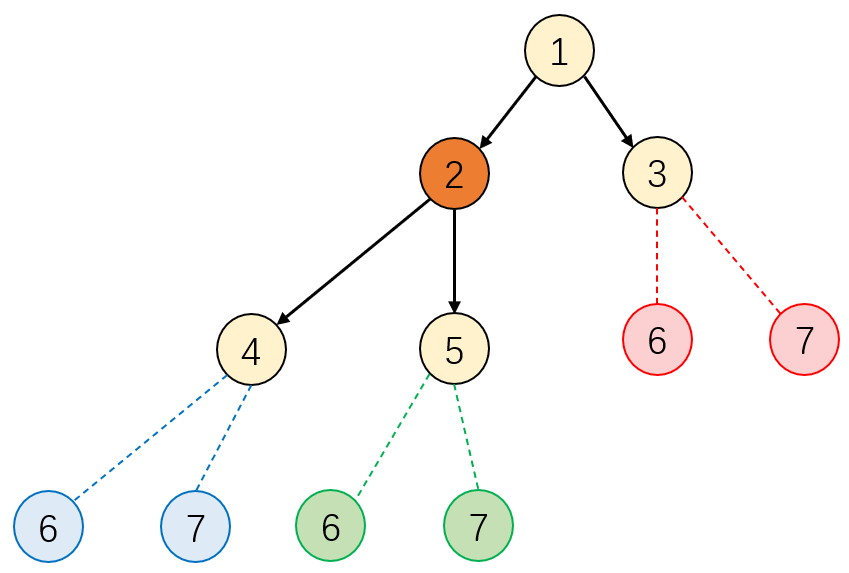
\includegraphics[width=5cm]{pic1.png}
\end{center}
\end{figure}
\end{frame}

\begin{frame}{分类树的节点分裂}
在sklearn中提供了两种生长模式,它们分别被称为深度优先生长和最佳增益生长,当参数max\_leaf\_nodes使用默认值None时使用前者,当它被赋予某个数值时使用后者。
\newline

深度优先生长采用深度优先搜索的方法:若当前节点存在未搜索过的子节点,则当前节点跳转到子节点进行分裂决策;若当前节点为叶节点,则调转到上一层节点,直到根节点不存在未搜索过的子节点为止。对上图而言,当前节点为2号,它的两个子节点4号和5号都没有被搜索过,因此下一步则选择两个节点中的一个进行跳转。在底层数据结构上,由于深度优先生长采用了“先进后出”的节点搜索模式,故使用栈(Stack)结构。当决策树使用最佳增益生长时,每次总是选择会带来最大相对信息增益的节点进行分裂,直到叶节点的最大数量达到max\_left\_nodes。

\end{frame}

\section{CART树}

\begin{frame}{CART树}
CART(Classification And Regression Tree)是一棵二叉树,它既能处理分类问题,又能够处理回归问题。值得注意的是,在sklearn中并没有实现处理类别特征和处理缺失值的功能,前者是因为多个类别的特征会产生多叉树,后者是因为sklearn认为用户应当自己决定缺失值的处理而不是交给模型来决定。
\newline

对于回归树而言,每个叶节点输出的不再是类别而是数值,其输出值为该叶节点所有样本标签值的均值。在每次分裂时,我们希望不同的子节点之间的差异较大,但每个子节点内部的差异较小。此时,分割策略仍然可以采用随机分割法或最佳分割法,只是现在不再以熵(条件熵)来评价节点(子节点)的纯度。
\end{frame}

\begin{frame}{CART树}
我们应当如何定义回归树的节点纯度?对于数值标签而言,我们可以认为节点间元素大小越接近则纯度越高,因此可以考虑使用均方误差(MSE)或平均绝对误差(MAE)来替换熵和条件熵的位置。
\newline

设节点$N$的样本标签为$y^{(D)}_1,...,y^{(D)}_N$,左右子节点的样本个数分别为$y^{(L)}_1,...,y^{(L)}_{N_R}$和$y^{(R)}_1,...,y^{(R)}_{N_R}$,记$\bar{y}^{(D)}=\frac{1}{N}\sum_{i=1}^{N}y^{(D)}_i$、$\bar{y}^{(L)}=\frac{1}{N_L}\sum_{i=1}^{N_L}y^{(L)}_i$和$\bar{y}^{(R)}=\frac{1}{N_R}\sum_{i=1}^{N_R}y^{(R)}_i$分别为节点$N$的样本标签均值、左子节点的样本标签均值和右子节点的样本标签均值,再记$\tilde{y}^{(D)}$、$\tilde{y}^{(L)}$和$\tilde{y}^{(R)}$分别为节点$N$的样本标签中位数、左子节点的样本标签中位数和右子节点的样本标签中位数。
\end{frame}
\begin{frame}{CART树}
此时,两者的信息增益可以分别定义为
\begin{align*}
G^{MSE}(X,Y)&=-\sum_{i=1}^{N}(y^{(D)}_i-\bar{y}^{(D)})^2+\frac{N_L}{N}\sum_{i=1}^{N_L}(y^{(L)}_i-\bar{y}^{(L)})^2\\
&\qquad+\frac{N_R}{N}\sum_{i=1}^{N_R}(y^{(R)}_i-\bar{y}^{(R)})^2
\end{align*}
\begin{align*}
G^{MAE}(X,Y)&=-\sum_{i=1}^{N}\vert y^{(D)}_i-\tilde{y}^{(D)}\vert+\frac{N_L}{N}\sum_{i=1}^{N_L}\vert y^{(L)}_i-\tilde{y}^{(L)}\vert\\
&\qquad+\frac{N_R}{N}\sum_{i=1}^{N_R}\vert y^{(R)}_i-\tilde{y}^{(R)}\vert
\end{align*}
\end{frame}

\begin{frame}{CART树}
当样本带有权重时,加权信息增益定义为
\begin{align*}
G_{\mathbf{w}}^{MSE}(X,Y)&=-\sum_{i=1}^{N}(y^{(D)}_i-\bar{y}^{(D)})^2+\frac{\sum_{i=1}^{N_L}w^{(N)}_i}{\sum_{i=1}^{N}w^{(N_L)}_i}\sum_{i=1}^{N_L}(y^{(L)}_i-\bar{y}^{(L)})^2\\
&\qquad+\frac{\sum_{i=1}^{N_R}w^{(N)}_i}{\sum_{i=1}^{N}w^{(N_R)}_i}\sum_{i=1}^{N_R}(y^{(R)}_i-\bar{y}^{(R)})^2
\end{align*}
\begin{align*}
G_{\mathbf{w}}^{MAE}(X,Y)&=-\sum_{i=1}^{N}\vert y^{(D)}_i-\tilde{y}^{(D)}\vert+\frac{\sum_{i=1}^{N_L}w^{(N)}_i}{\sum_{i=1}^{N}w^{(N_L)}_i}\sum_{i=1}^{N_L}\vert y^{(L)}_i-\tilde{y}^{(L)}\vert\\
&\qquad+\frac{\sum_{i=1}^{N_R}w^{(N)}_i}{\sum_{i=1}^{N}w^{(N_R)}_i}\sum_{i=1}^{N_R}\vert y^{(R)}_i-\tilde{y}^{(R)}\vert
\end{align*}
\end{frame}

\begin{frame}{CART树}
当处理分类问题时,虽然ID3或C4.5定义的熵仍然可以使用,但是由于对数函数$\log$的计算代价较大,CART将熵中的$\log$在$p=1$处利用一阶泰勒展开,基尼系数定义为熵的线性近似,即由于
$$
H(X)=\mathbbm{E}_XI(p)=\mathbbm{E}_X[-\log_2p(X)]\approx\mathbbm{E}_X[1-p(X)]
$$
从而定义基尼系数为
\begin{align*}
{\rm Gini}(X)&=\mathbbm{E}_X[1-p(X)]\\
&=\sum_{k=1}^K \tilde{p}(x_k)(1-\tilde{p}(x_k))\\
&=1-\sum_{k=1}^K\tilde{p}^2(x_k)
\end{align*}
\end{frame}
\begin{frame}{CART树}
类似地定义条件基尼系数为
\begin{align*}
{\rm Gini}(X\vert Y)&=\mathbbm{E}_Y[\mathbbm{E}_{X\vert Y}1-p(X\vert Y)]\\
&=\sum_{m=1}^M \tilde{p}(y_m)\sum_{k=1}^K[\tilde{p}(x_k\vert y_m)(1-\tilde{p}(x_k\vert y_m))]\\
&=\sum_{m=1}^M \tilde{p}(y_m)[1-\sum_{k=1}^K\tilde{p}^2(x_k\vert y_m)]
\end{align*}
从而引出基于基尼系数的信息增益为
$$
G(X,Y)={\rm Gini}(X)-{\rm Gini}(X\vert Y)
$$
\end{frame}
\section{决策树的剪枝}

\begin{frame}{决策树的剪枝}
决策树具有很强的拟合能力,对于任何一个没有特征重复值的数据集,决策树一定能够在训练集上做到分类错误率或均方回归损失为0,因此我们应当通过一些手段来限制树的生长,这些方法被称为决策树树的剪枝方法。其中,预剪枝是指树在判断节点是否分裂的时候就预先通过一些规则来阻止其分裂,后剪枝是指在树的节点已经全部生长完成后,通过一些规则来摘除一些子树。
\newline

在sklearn的CART实现中,一共有6个控制预剪枝策略的参数,它们分别是最大树深度max\_depth、节点分裂的最小样本数min\_samples\_split、叶节点最小样本数min\_samples\_leaf、节点样本权重和与所有样本权重和之比的最小比例min\_weight
\_fraction\_leaf、最大叶节点总数max\_leaf\_nodes以及之前提到的分裂阈值min\_impurity\_decrease。
\end{frame}

\begin{frame}{决策树的剪枝}
后剪枝过程又称作MCCP过程,即Minimal Cost-Complexity Pruning,它由参数ccp\_alpha控制,记其值为$\alpha$。一般而言,树的叶子越多就越复杂,为了抑制树的生长,我们定义以节点$N$为根节点的树$T^N$的复杂度为该树的叶节点数量$\vert T^N\vert$。设树$T$的剪枝度量为
$$R_\alpha(T^N)=R(T^N)+\alpha\vert T^N\vert $$
其中,$R(T^N)$代表各个叶子节点的条件熵/条件基尼系数之和(分类问题)或均方误差/平均绝对误差之和(回归问题),即MCCP中的Cost部分,$\alpha\vert T^N\vert$对应的就是Complexity部分。
\end{frame}

\begin{frame}{决策树的剪枝}
对于树的单个节点而言,由于此时节点数为1,故其剪枝度量为$R_\alpha(Node^N)=R(Node^N)+\alpha$。树剪枝的思想在于,如果对于决策树某一个节点为根的子树,其根的剪枝度量低于该子树的剪枝度量,那么这个根节点就没有必要分裂,即砍掉这棵子树中除了根节点以外的所有节点。
\newline

此时,我们可以得到剪枝的依据为
$$
R_{\alpha}(Node^N)\leq R_{\alpha}(T^N)
$$
这等价于

$$
R(Node^N)+\alpha \leq R(T^N) + \alpha \vert T^N\vert
$$
\end{frame}
\begin{frame}{决策树的剪枝}
对上式进行移项后可得
$$
E(Node^N) = \frac{R(Node^N)-R(T)}{\vert T^N\vert -1}\leq \alpha
$$
这个条件表明只要$E(Node^N)$的值小于给定的参数cpp\_alpha,那么这个节点下的所有节点都会被删除。事实上在sklearn中,在树完全生成后就会把所有节点的$E(Node^N)$值进行记录,每次剪枝都会分别查看所有非叶子节点的树节点对应的$E(Node^N)$值,并且对具有最小$E(Node^N)$值的非叶子节点进行剪枝,直到所有节点的$E(Node^N)$值都大于给定的cpp\_alpha。
\end{frame}
\section{习题}

\begin{frame}[allowframebreaks]{习题(A)}
\begin{enumerate}
\item ID3树算法、C4.5树算法和CART算法之间有何异同?
\item 什么是信息增益率?它衡量了什么指标?它有什么缺陷?
\item sklearn决策树中的random\_state参数控制了哪些步骤的随机性?
\item 决策树如何处理连续变量和缺失变量?
\item 基尼系数是什么?为什么要在CART中引入它?
\item 什么是树的预剪枝和后剪枝?具体分别是如何操作的?
\end{enumerate}
\end{frame}

\begin{frame}[allowframebreaks]{习题(B)}
\begin{enumerate}
\item 在一般的机器学习问题中,我们总是通过一组参数来定义模型的损失函数,并且在训练集上以最小化该损失函数为目标进行优化。请问对于决策树而言,模型优化的目标是什么?
\item 如何理解min\_samples\_leaf参数能够控制回归树输出值的平滑程度?
\item 我们在第4节提到决策树具有很强的拟合能力,对于任何一个没有特征重复值的数据集,它一定能够在训练集上做到分类错误率或均方回归损失为0。为什么?
\item 为什么采用深度优先生长策略的决策树应当使用“先进先出”的策略?
\framebreak
\item 对信息熵中的$\log$函数在$p=1$处进行一阶泰勒展开可以近似为基尼系数,那么如果在$p=1$处进行二阶泰勒展开我们可以获得什么近似指标?请写出对应指标的信息增益公式。
\item 除了信息熵和基尼系数之外,我们还可以使用节点的$$1-\max_{k}p(X=x_k)$$和第$m$个子节点的$$1-\max_{k}p(X=x_k\vert Y=y_m)$$来作为衡量纯度的指标。请解释其合理性并给出相应的信息增益和加权信息增益公式。
\framebreak
\item 在讨论缺失值对信息增益的惩罚时,我们直接使用了$1-\gamma$作为惩罚系数,其中$\gamma$为缺失值的比例。如果将系数替换为$1-\gamma^2$,请问对缺失值而言是加强了惩罚还是削弱了惩罚?
\item 如果将树的生长策略从深度优先生长改为广度优先生长,假设其他参数保持不变的情况下,两个模型对应的结果输出可能不同吗?
\item 请实现参数与sklearn一致的DecisionTreeClassifier类,其成员函数包括fit、predict和predict\_proba,同时需给出feature\_importances\_指标。
\begin{itemize}
\item predict\_proba返回的是测试样本所在叶节点的各类别比例。
\item feature\_importances\_指每个特征的重要性,对于某个特征而言,其特征重要性等于决策树中根据该特征分裂而产生的相对信息增益之和。
\end{itemize}
\framebreak
\item 假设当前我们需要处理一个分类问题,请问对输入特征进行归一化会对树模型的类别输出产生影响吗?请解释原因。
\item sklearn提供了class\_weight参数来处理非平衡样本。设每个类别的样本数量为$n_1,...,n_K$,第$i$个样本的类别、样本权重和类别权重分别为$k$、$w_i$和$w^c_i$。当class\_weight值是形式为\{class\_label: class\_weight\}的字典时,样本权重被调整为$w_i\cdot w^c_i$;当class\_weight值是字符串“balanced”,样本权重被调整为$w_i\cdot \frac{\sum_{k'=1}^K n_{k'}}{K\cdot n_k}$;否则$w_i$不变。现有样本$x_1$、$x_2$和$x_3$的样本权重为$[20,30,10]$,类别分别是$0$、$0$和$1$,且给定class\_weight=\{0:40, 1:60\},请计算调整后的样本权重。
\framebreak
\item $X,Y$的联合熵为$H(X,Y)=\mathbbm{E}_{(X,Y)\sim p(x,y)}[-\log_2p(X,Y)]$
\begin{itemize}
\item 请证明如下关系:
\begin{itemize}
\item $G(X,Y)=H(Y)-H(Y\vert X)$
\item $G(X,Y)=H(X)+H(Y)-H(X,Y)$
\item $G(X,Y)=H(X,Y)-H(X\vert Y)-H(Y\vert X)$
\end{itemize}
\item 下图被分为了A、B和C三个区域。若AB区域代表X的不确定性,BC区域代表Y的不确定性,那么$H(X)$、$H(Y)$、$H(X\vert Y)$、$H(Y\vert X)$、$H(X,Y)$和$G(X,Y)$分别指代的是哪片区域?
\end{itemize}
\begin{figure}
\begin{center}
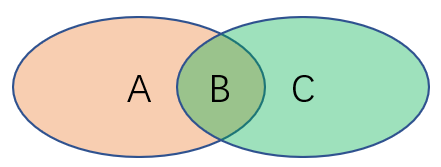
\includegraphics[width=3.5cm]{pic3.png}
\end{center}
\end{figure}
\end{enumerate}
\end{frame}

\begin{comment}

\section{一些例子}

\begin{frame}[fragile]{$\rm E$ $\rm Step$}
\begin{align*}
\mathbb{E}_{\bm{Z}\sim q^*}[z_{ij}]&= p(z_{ij}=1)\times 1 + p(z_{ij}=0)\times 0\\
&= \frac{\pi_j^{now}{{\rm N}(\bm{x_i}\vert \bm{\mu_j}^{now},\bm{\Lambda_j}^{now})}}{\sum_{j=1}^k\pi_{j}^{now}{\rm N}(\bm{x_i}\vert \bm{\mu_j}^{now}, \bm{\Lambda_j}^{now})}
\end{align*}
\begin{lstlisting}
def z_compute(_pi, _mu_1, _mu_2, _sigma_1, _sigma_2):
    res = np.c_[
            multivariate_normal.pdf(X, mean=mu_1, cov=sigma_1),
            multivariate_normal.pdf(X, mean=mu_2, cov=sigma_2)
        ]
    res = res * _pi
    res = res / res.sum(1).reshape(-1,1)
    return res
\end{lstlisting}

\end{frame}

\end{comment}


\end{document}